\chapter{Κανονικοποίηση}
\label{appendix:Reg}
\paragraph{Διακύμανση - Πόλωση Μοντέλου}
Κατά την επιλογή του μοντέλου που θα χρησιμοποιήσουμε για μια εφαρμογή μηχανικής μάθησης, το βασικό δίλημμα μπροστά στο οποίο βρισκόμαστε είναι αυτό της πολυπλοκότητας της υπόθεσης. Το γεγονός πως προσπαθούμε να προσεγγίσουμε μία άγνωστη συνάρτηση και η αμφιβολία που νιώθουμε για την αξιοπιστία των δεδομένων μας καθιστούν τη λήψη της απόφασης ενστικτώδη και ριψοκίνδυνη. Στο παρακάτω παράδειγμα, έχουμε κάποια δισδιάστατα δεδομένα για ένα πρόβλημα παλινδρόμησης και θέλουμε να επιλέξουμε μεταξύ δύο μοντέλων:
\begin{figure}[H]
	\centering			
%	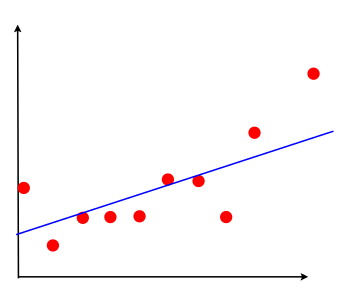
\includegraphics[width=0.6\textwidth, height=5cm]{bias.png}
	\caption[Μοντέλο υψηλής πόλωσης]{Μοντέλο υψηλής πόλωσης}
\end{figure}
Η πρώτη επιλογή μας συνιστά μία ευθεία, δηλαδή ένα πολυώνυμο πρώτης τάξης, το οποίο καθορίζεται από δύο παραμέτρους. Παρατηρούμε πως το μοντέλο αυτό είναι τόσο απλό, που όσο και να προσπαθήσουμε δε θα καταφέρει να προβλέψει καλά τα δεδομένα μας. Θα ήταν ουτοπικό να χαρακτηρίζεται κάποιο πραγματικό φαινόμενο από μια τόσο απλή συνάρτηση, οπότε θα απορρίπταμε αυτό το μοντέλο ως υψηλά πολωμένο, καθώς κάνει μια σημαντική υπόθεση απλότητας.
\begin{figure}[H]
	\centering			
%	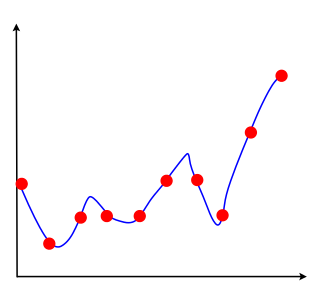
\includegraphics[width=0.6\textwidth, height=5cm]{variance.png}
	\caption[Μοντέλο υψηλής διακύμανσης]{Μοντέλο υψηλής διακύμανσης}
\end{figure}
Η δεύτερη επιλογή μας είναι ένα πολυώνυμο υψηλής τάξης, το οποίο μπορεί εύκολα να επιδείξει μηδενικό σφάλμα στα δεδομένα εκπαίδευσης που διαθέτουμε. Το μοντέλο αυτό είναι φαινομενικά τέλειο και αναπόφευκτα προκαλεί αμφιβολίες: είναι όλα τα δεδομένα μας τόσο αξιόπιστα και χαρακτηριστικά για το φαινόμενο που προβλέπουμε, ώστε να αξίζει να τα προσεγγίσουμε τέλεια; Γενικά, δεδομένα πολύ υψηλής διακύμανσης είναι ύποπτα για θόρυβο, ο οποίος ως τυχαίος είναι συχνά υψίσυχνος, σε αντίθεση με φυσικά δεδομένα που υπακούν σε κάποιες συνθήκες ομαλότητας. Μήπως λοιπόν στην προσπάθειά μας να προβλέψουμε καλά την άγνωστη συνάρτηση παρασυρθήκαμε και μοντελοποιήσαμε το θόρυβο; Ένα τέτοιο μοντέλο είναι καταδικασμένο να αποτύχει σε καινούρια δεδομένα και χαρακτηρίζεται ως μοντέλο υψηλής διακύμανσης. Το παραπάνω πρόβλημα είναι αυτό που έχουμε αποκαλέσει υπερπροσαρμογή.

Ο θόρυβος, που μας παρασύρει σε υπερπροσαρμογή, αποτελείται από δύο συνιστώσες: το στοχαστικό θόρυβο, ο οποίος κάθεται τυχαία στα δεδομένα μας και χαρακτηρίζεται από μία κατανομή $\epsilon(x)$ και τον ντετερμινιστικό. Ο τελευταίος οφείλεται στην πολυπλοκότητα της συνάρτηση-στόχου: το μοντέλο ερμηνεύει ως θόρυβο οποιαδήποτε διακύμανση δεν μπορεί να μοντελοποιήσει, καθώς είναι πολύ πολύπλοκη για αυτό, είτε αυτή γεννήθηκε τυχαία είτε προήλθε από τη συνάρτηση-στόχο.

Η μαθηματική αποτύπωση του παραπάνω προβλήματος έχει ως εξής: αν επιλέξουμε ένα μοντέλο $g(x)$ για να προβλέψουμε μια συνάρτηση $f(x)$ και ορίσουμε ως $\bar{g(x)}$ την καλύτερη δυνατή πρόβλεψη που μπορεί να κάνει το μοντέλο δεδομένων των παραμέτρων που περιέχει και της πολυπλοκότητας της $f(x)$ και $g_D(x)$ όλες τις πιθανές υποθέσεις που είναι σε θέση να κάνει το μοντέλο, ρυθμίζοντας τις παραμέτρους του, τότε το σφάλμα στο σετ εκπαίδευσης μπορεί να χαρακτηρισθεί ως εξής:
$$E_{error}=\underbrace{E_x(g_D(x) - g(x))^2}_{\text{σφάλμα λόγω  διακύμανσης}} + \underbrace{E_x(g(x)- f(x))^2}_{\text{σφάλμα λόγω πόλωσης}} + E_{\epsilon,x}(\epsilon(x^2))$$
\paragraph{Η ιδέα της κανονικοποίησης} Η τεχνική της κανονικοποίησης στοχεύει στη μείωση της διακύμανσης με ταυτόχρονη διατήρηση χαμηλής πόλωσης. Με απλά λόγια, προσπαθεί να διατηρήσει την πολυπλοκότητα της υπόθεσης, διατηρώντας το
ίδιο πλήθος παραμέτρων, ώστε να έχει τη δυνατότητα να προβλέψει μια πολύπλοκη συνάρτηση-στόχο, περιορίζοντας ωστόσο την επιλογή των τιμών των παραμέτρων, ώστε να δυσκολεύεται να προβλέψει το θόρυβο.
\begin{figure}[H]
	\centering			
%	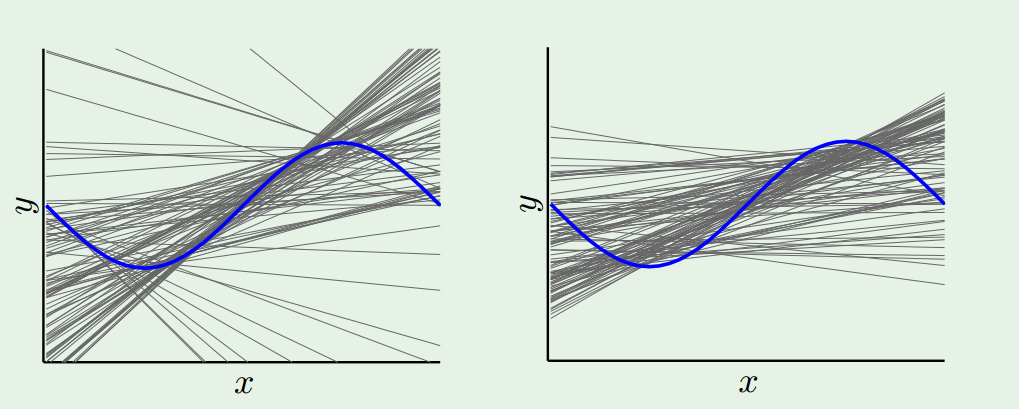
\includegraphics[width=0.8\textwidth]{reg_example.png}
	\caption[Παράδειγμα κανονικοποίησης]{Παράδειγμα κανονικοποίησης: Η άγνωστη συνάρτηση που προσπαθούμε να προβλέψουμε είναι ένα ημίτονο και το μοντέλο που επιλέγουμε είναι το γραμμικό, για χάρη απλότητας. Αριστερά, πριν την κανονικοποίηση, το μοντέλο μας είναι ελεύθερο να επιλέξει οποιαδήποτε ευθεία επιθυμεί. Δεξιά, έχουμε περιορίσει την κλίση και το σταθερό συντελεστή της ευθείας, καταφέρνοντας μικρότερη διακύμανση στις υποθέσεις μας και μικρότερο σφάλμα, καθώς έχουν αποκλειστεί κάποιες πολύ κακές υποθέσεις.}
\end{figure}

Στη συνέχεια θα δούμε πώς εφαρμόζεται η κανονικοποίηση σε ένα πρόβλημα λογιστικής παλινδρόμησης με πολυωνυμικό μοντέλο και θα κατανοήσουμε την επίλυση γραφικά.

Όπως έχουμε δει στο κεφάλαιο της λογιστικής παλινδρόμησης, η συνάρτηση λάθους που προσπαθούμε να ελαχιστοποιήσουμε ώστε να βρούμε τη βέλτιστη υπόθεση είναι η εξής:
$$E_{in}(w)=\frac{1}{N} \sum_{n=1}^{N} (w^T z_n  - y_n)^2$$

όπου w είναι οι συντελεστές του μοντέλου, y το διάνυσμα κλάσης και x τα διανύσματα εισόδου των Ν παραδειγμάτων. Η λύση της παραπάνω εξίσωσης είναι:
$$w_{in}=(Z^T \inv{Z} y)$$

Αν ορίσουμε την προσπάθειά μας να περιορίσουμε τις παραμέτρους ως τοποθέτηση ενός άνω φράγματος στο μέτρο των συντελεστών, τότε το αναδιατυπωμένο, κανονικοποιημένο πλέον, πρόβλημα έχει ως εξής:
\begin{flalign*}
\text{Ελαχιστοποίηση} && E_{in}(w)=\frac{1}{N} (Zw-y)^T (Zw-y)  &&\\
\text{Υπό τον περιορισμό} && w^T w \leq C  &&
\end{flalign*}

Το παραπάνω πρόβλημα καθιστά πρόβλημα βελτιστοποίησης με περιορισμό που περιέχει ανισότητα, επομένως μπορεί να επιλυθεί με πολλαπλασιαστές Lagrane και τη βοήθεια της θεωρίας Karush-Kuhn- Tucker. Ωστόσο η γραφική αναπαράσταση του προβλήματος ενδεχομένως να είναι ενδιαφέρουσα, καθώς θα δώσει καλύτερη κατανόηση της φύσης του.

Όπως έχουμε δει στο κεφάλαιο της λογιστικής παλινδρόμησης, η εξίσωση του σφάλματος έχει τη μορφή ελλειψοειδούς καμπύλης. Ο περιορισμός που θέσαμε ορίζει έναν κύκλο στον οποίο κινούνται τα επιτρεπτά w, με ακτίνα C.
\begin{figure}[H]
	\centering			
%	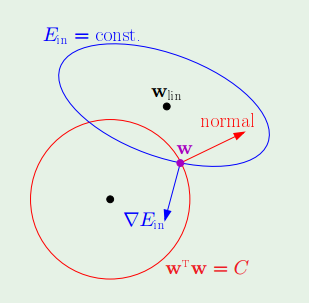
\includegraphics[scale=0.7]{opt_graph.png}
	\caption[Γραφική αναπαράσταση κανονικοποίησης]{Γραφική αναπαράσταση κανονικοποίησης.}
\end{figure}
H πληροφορία της κατεύθυνσης προς την οποία πρέπει να κινηθούμε, ώστε να μειώσουμε το $E_{in}$ δίνεται ως γνωστόν από την κλίση, $\nabla E_{in}$ στο σημείο που βρισκόμαστε και φαίνεται στο παραπάνω σχήμα. Όσο αφορά τα w, είναι διανύσματα που κινούνται πιο κοντά γίνεται στη βέλτιστη λύση $w_{lin}$, παραμένοντας βέβαια στον κύκλο. Στο σχήμα φαίνεται πως στην καλύτερη περίπτωση βρίσκονται πάνω στην περιφέρειά του. Παρατηρώ πως, επειδή μεταξύ των δύο διανυσμάτων υπάρχει γωνία, καθώς κινούμαι στον κύκλο, το σφάλμα θα αυξομειώνεται και επομένως δε θα το βελτιστοποιώ. Αντιθέτως, αν το w πάρει την αντίθετη κατεύθυνση από το  $\nabla E_{in}$, θα κινούμαι προς τη βέλτιστη λύση. Επομένως ορίζω τη συνθήκη:
$$\nabla E_{in}= - 2 \frac{\lambda}{N} w_{reg}$$
όπου  ως $w_{reg}$ συμβολίζονται οι κανονικοποιημένοι πλέον συντελεστές, $\lambda$ μια σταθερή παράμετρος που επηρεάζει την κανονικοποίηση και N, το γνωστό μας πλήθος παραδειγμάτων.

Σκεπτόμενοι αντιστρόφως από ότι συνήθως, παρατηρούμε πως η παραπάνω εξίσωση μοιάζει με μηδενισμό της παραγώγου μιας συνάρτησης και επομένως θα μπορούσε να αποτελέσει την προσπάθεια βελτιστοποίησης του παρακάτω προβλήματος:
$$E_{in} + \frac{\lambda}{N} w^T_{reg} w_{reg}=0$$

Η παραπάνω διατύπωση είναι αποκαλυπτική: ένα πρόβλημα βελτιστοποίησης υπό συνθήκη αναδιατυπώθηκε ως ένα απλό πρόβλημα βελτιστοποίησης μιας συνάρτησης, που αντικαθιστώντας με τη γνωστή μας συνάρτηση του $E_{in}$ εκφράζεται ως:
$$E_{in}(w)=\frac{1}{N}(Zw-y)^T(Zw-y) + \frac{\lambda}{N} w^T_{reg} w_{reg} $$

Με τη ίδια λογική, που είχαμε επιλύσει το πρόβλημα χωρίς κανονικοποίηση, το ψευδοαντίστροφο, η λύση προκύπτει ως:
$$w_{lin}=\inv{ (Z^T Z)} Z^T y$$

Αν και είδαμε την εφαρμογή της κανονικοποίησης σε ένα συγκεκριμένο μοντέλο, μπορούμε να κατανοήσουμε τη συνολική διαδικασία ως εξής:

$$E_{aug}(h)= E_{in}(h) + \frac{\lambda}{N} \Omega(h)=0$$

όπου ως $E_{in(h)}$ συμβολίζουμε το σφάλμα μιας υπόθεσης πριν την κανονικοποίηση και $E_{aug}(h)$ το επαυξημένο σφάλμα, δηλαδή έπειτα από την κανονικοποίηση. Η συνάρτηση $\Omega(h)$ εκφράζει τον τρόπο που θα γίνει η κανονικοποίηση και, ανεξάρτητα από το μοντέλο, έχει ως στόχο την επιβολή περιορισμών που εξασφαλίζουν ομαλότητα ή/και χαμηλότερη πολυπλοκότητα της υπόθεσης.
\paragraph{Η επίδραση της παραμέτρου λ}
Αν η συνάρτηση $\Omega(h)$ εκφράζει τον τρόπο, τότε το $\lambda$ εκφράζει το μέγεθος της κανονικοποίησης.
\begin{figure}[H]
	\centering			
%	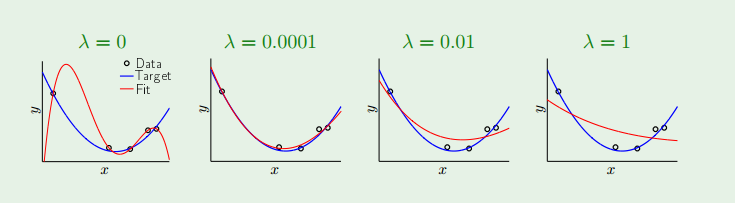
\includegraphics[width=0.8\textwidth]{l_reg.png}
	\caption[Επίδραση λ στην κανονικοποίηση]{Επίδραση λ στην κανονικοποίηση.}
\end{figure}

Όπως παρατηρούμε στο παραπάνω διάγραμμα υποπεριπτώσεων, επιβολή μικρής τιμής $\lambda$, αντιστοιχεί σε μεγάλο C, δηλαδή ασθενή περιορισμό του μοντέλου, που συνεχίζει να κινδυνεύει από υπερπροσαρμογή. Καθώς αυξάνουμε την τιμή του $\lambda$ γινόμαστε αυστηρότεροι, με κίνδυνο να είμαστε τόσο περιοριστικοί με το μοντέλο που θα οδηγηθούμε σε υπόθεση υψηλής πόλωσης.

